\documentclass[a4paper,11pt]{article}

\usepackage{amsfonts}
\usepackage{amsmath}
\usepackage{amssymb}
\usepackage{graphicx}

\usepackage[utf8]{inputenc}
\usepackage[T1]{fontenc}

\title{Projekt Egzaminacyjny}
\author{Jan Milewczyk, Maciej Wojciechowski, Kajetan Lach}

\begin{document}

\maketitle

\section{Analizy log-zwrotów spółek}

\subsection{Vigo Photonics}

\subsubsection{Wstęp}
\textbf{Vigo Photonics} to polskie przedsiębiorstwo specjalizujące się w wytwarzaniu materiałów i przyrządów półprzewodnikowych do zastosowań fotonicznych i mikroelektronicznych. Spółka jest liderem na światowym rynku fotonowych detektorów średniej podczerwieni, a wszystkie produkty opiera na własnej, unikalnej technologii.

\subsubsection {Analiza log-zwrotów spółki (Vigo Photonics)}
Pierwszy rozdział zawiera analizę log-zwrotów spółki.


\newpage\paragraph{Wykresy kursów zamknięcia oraz log-zwrotów:}
Poniższy wykres ilustruje zmianę cen zamknięcia akcji w czasie.

\centerline{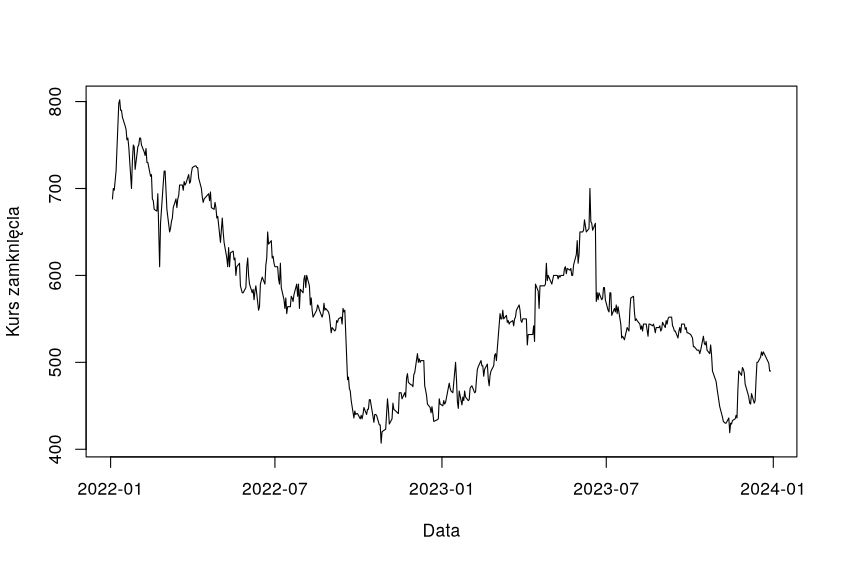
\includegraphics[width=1\textwidth]{./Kajtek/img/kursy_zamkniecia_plot.png}}

Zmianę log-zwrotów, wyliczonych według wzoru

$$ r_1 = \ln\frac{S_0}{S_1}, r_2 = \ln\frac{S_2}{S_1}, ..., r_n = \ln\frac{S_n}{S_{n-1}} $$

gdzie $s_0, s_1, ..., s_n$ są kursami zamknięcia z kolejnych dni, na osi czasu ilustruje wykres poniżej.

\centerline{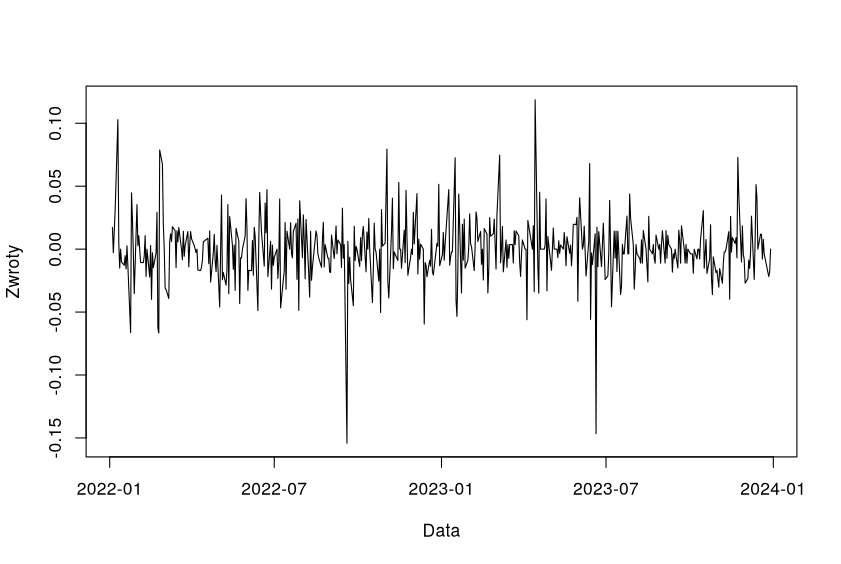
\includegraphics[width=1\textwidth]{./Kajtek/img/log_zwroty_plot.png}}


\paragraph{Wartość oczekiwana:}
Zakładając, że log-zwroty $r_1, r_2, ..., r_n$ są niezależnymi realizacjami zmiennej losowej X, wyliczamy $\mu$ przy użyciu nieobciążonego estymatora wartości oczekiwanej:
$$ E(\overline{X}_n) = \frac{1}{n}\sum_{i=1}^{n}X_i = \mu $$
w wyniku czego otrzymujemy wynik 
$$\mu = -0.0006787669$$


\paragraph{Wariancja i odchylenie standardowe:}
Korzystając ze wzoru na nieobciążony estymator wariancji
$$\sigma^{2}=\frac{1}{n-1}\sum_{i=1}^{n}(X_i - \overline{X}_n)^{2}$$
otrzymujemy $\sigma^{2}=0.0006189792$ oraz $\sigma=0.02487929$.
\paragraph{Kwantyle:}
Z wykorzystaniem klasycznego estymatora kwantyli wyestymowano kwantyle rzędu $\alpha = 5\%, 50\% i 95\%$. Wyniki przedstawione zostaly w tabeli poniżej:
\begin{center}
\begin{tabular}{|c|c|c|c|c|c|}
    \hline
    $\overline{x}_n$ & $s_n^{2}$ & $s_n$ & $q(5\%)$ & $q(50\%)$ & $q(95\%)$ \\ \hline
    -0.0006787669 & 0.0006189792 & 0.02487929 & -0.03620640 & 0 & 0.04055989 \\ \hline
\end{tabular}
\end{center}


\paragraph{Histogram log-zwrotów:}
Na histogramie dziennych log-zwrotów cen akcji na czerwono i niebiesko oznaczono odpowiednio wartość wyestymowanej średniej oraz wartości kwantyli przedstawionych wcześniej.

\centerline{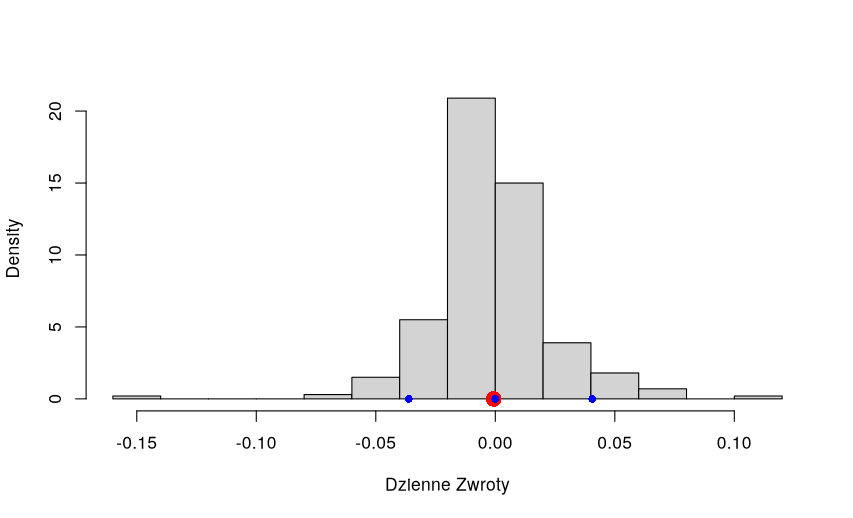
\includegraphics[width=1\textwidth]{./Kajtek/img/histogram_zwrotow.png}}


\newpage
\paragraph{Dystrybuanta:}
Z wykorzystaniem dystrybuanty empirycznej jako nieobciążonego estymatora 

$$\hat{F}_n(x) = \frac{1}{n} \sum_{i=1}^{n} 1_\{x_i \leq x\} = \left(\frac{\text{liczba  elementów  w  próbie} \leq x}{n}\right)$$
estymujemy dystrybuantę F zaprezentowaną na wykresie poniżej

\centerline{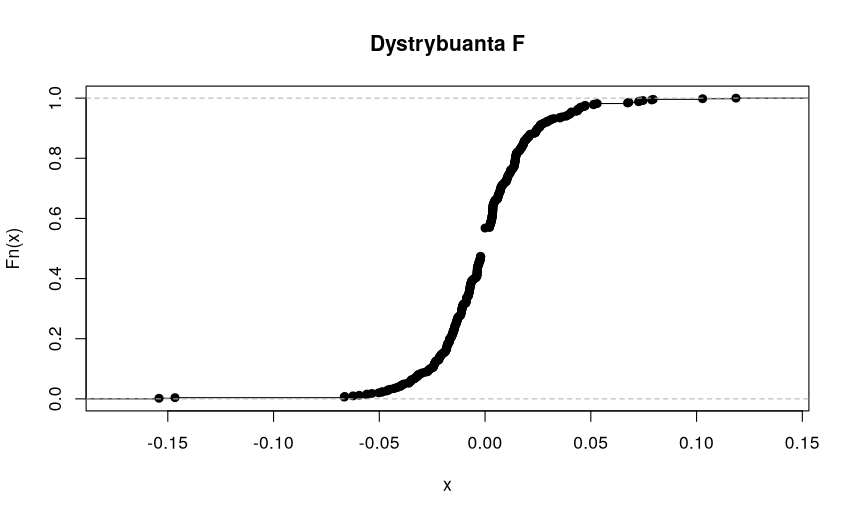
\includegraphics[width=1\textwidth]{./Kajtek/img/dystrybuanta.png}}

\paragraph{Analiza dobroci dopasowania rozkładu normalnego i t-Studenta:}
Korzystając z \textbf{estymatora największej wiarygodności (MLE)} parametru estymujemy parametry rozkładu normalnego i t-Studenta.

% zapisac tu wzory
\begin{center}
\begin{tabular}{|c|c|c|}
    \hline
    $m$ & $s$ & $df$ \\ \hline
    -0.0006787669 & 0.0248544 & 314.3698 \\ \hline
\end{tabular}
\end{center}

\newpage
\subsubsection{Wykresy diagnostyczne}
Poniższe wykresy prezentują kolejno porównania: histogram-gęstość wybranych rozkładów, kwantyl-kwantyl, dystrybuanta empiryczna-dystrybuanta teoretyczna wybranych rozkładów oraz prawdopodobieństwo teoretyczne wybranych rozkładów-prawdopodobieństwo empiryczne.

\centerline{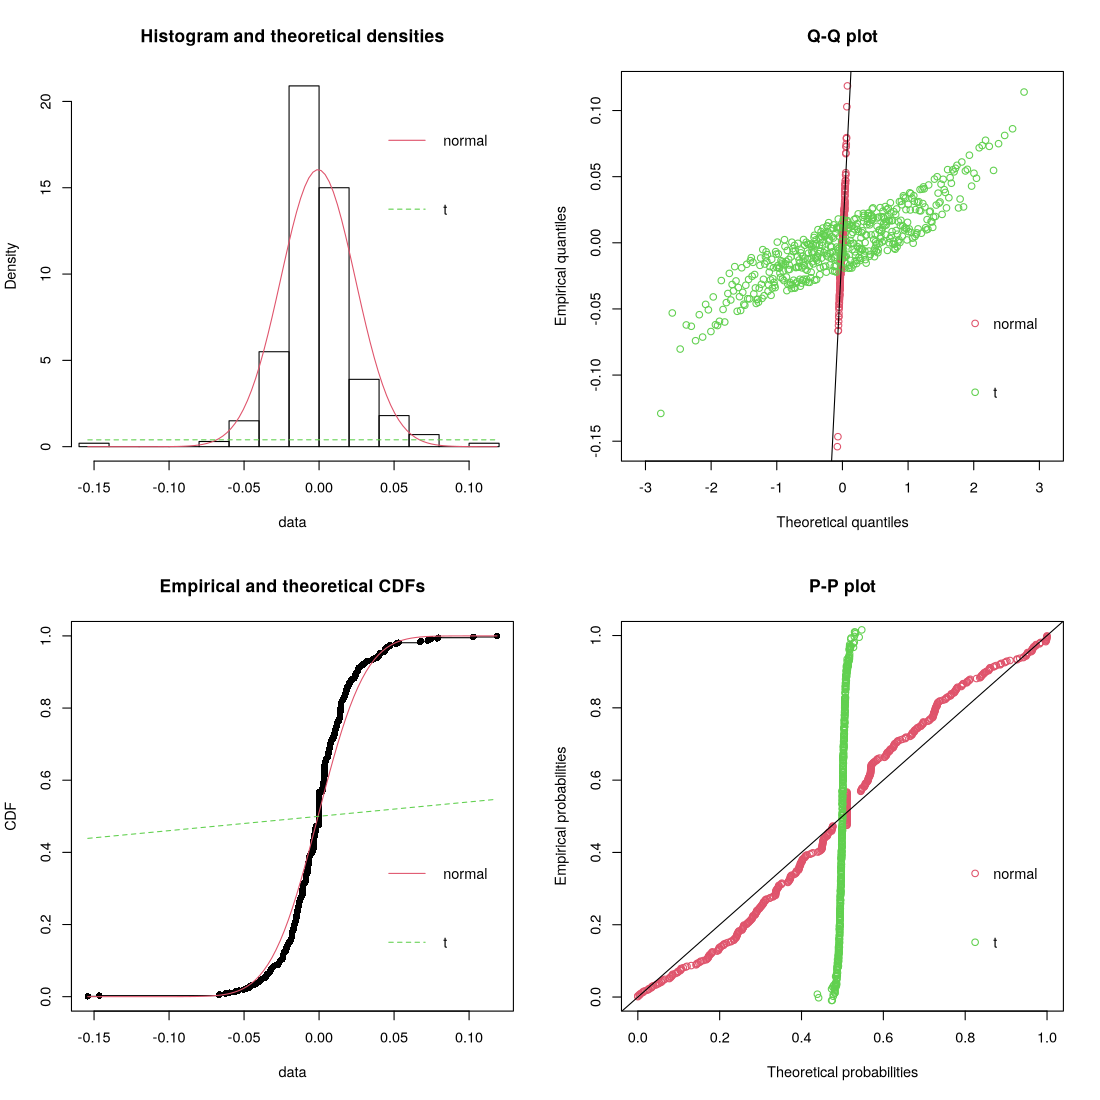
\includegraphics[width=1\textwidth]{./Kajtek/img/diagnostical-plots.png}}

Na ich podstawie można stwierdzić, że rozkład normalny lepiej dopasowuje się do danych.


\newpage
\paragraph{Weryfikacja wyboru z wykorzystainem statystyk oraz kryteriów informacyjnych:}
Poniższe tabele prezentują wyniki testów statystycznych oraz kryteriów informacyjnych dla rozkładów normalnego i t-Studenta.

\begin{center}
\begin{tabular}{|c|c|c|}
    \hline
    Statystyki & Rozkład normalny & Rozkład t-Studenta  \\ \hline
    Kolmogorov-Smirnov & 0.08251589 & 0.469477 \\ \hline
    Cramer-von Mises & 1.18780300 & 39.177553 \\ \hline
    Anderson-Darling & 6.95700925 & 183.184800 \\ \hline
\end{tabular}
\end{center}

\begin{center}
\begin{tabular}{|c|c|c|}
    \hline
    Kryteria & Rozkład normalny & Rozkład t-Studenta  \\ \hline
    AIC & -2271.782 & 922.0439 \\ \hline
    BIC & -2263.353 & 926.2585 \\ \hline
\end{tabular}
\end{center}

Powyższe wyniki potwierdzają, że rozkład normalny lepiej dopasowuje się do danych.


\paragraph{Test hipotezy równości rozkładów metodą Monte Carlo:}
Testujemy hipotezę zerową o równości dystrybuant
$$H_0: F = F_0$$
przeciwko hipotezie alternatywnej (kontrhipotezie)
$$H_1: F \neq F_0$$
gdzie $F_0$ jest dystrybuantą rozkładu normalnego wybranego w poprzedniej podsekcji, a F dystrybuantą nieznaną.
\newline Do przetestowania hipotezy zerowej o równości dystrybuant wykorzystamy metodę Monte Carlo przy użyciu statystyki Kołmogorowa-Smirnowa. 
\newline W tym celu generujemy $N=10000$ prób z rozkładu normalnego o parametrach 
$$m = -0.0006787669 \text{ oraz } s = 0.0248544$$ 
wyestymowanych wcześniej oraz obliczamy wartość statystyki Kołmogorowa-Smirnowa dla każdej z nich. 
\newline Następnie obliczamy prawdopodobieństwo 
$$p = P(D_n > d_n)$$ 
gdzie $D_n$ to wartość statystyki dla wygenerowanych prób a $d_n$ to jej wartość dla log-zwrotów spółki. 
\newline Ustalamy poziom istotności $\alpha = 0.05$ i sprawdzamy czy $p < \alpha$. W naszym przypadku 
$$p = 0.0025 < \alpha = 0.05$$ 
co pozwala nam odrzucić hipotezę zerową na rzecz hipotezy alternatywnej.

\subsection{Digitree}

\subsubsection{Wstęp}
Digitree to polska spółka technologiczna specjalizująca się w kompleksowych rozwiązaniach z zakresu digital marketingu i wsparcia sprzedaży online.


\subsubsection{Analiza log-zwrotów spółki DIGITREE}

\paragraph{Spółka DIGITREE:}
Poniżej przedstawiam wykres kursów zamknięcia wybranej spółki

\centerline{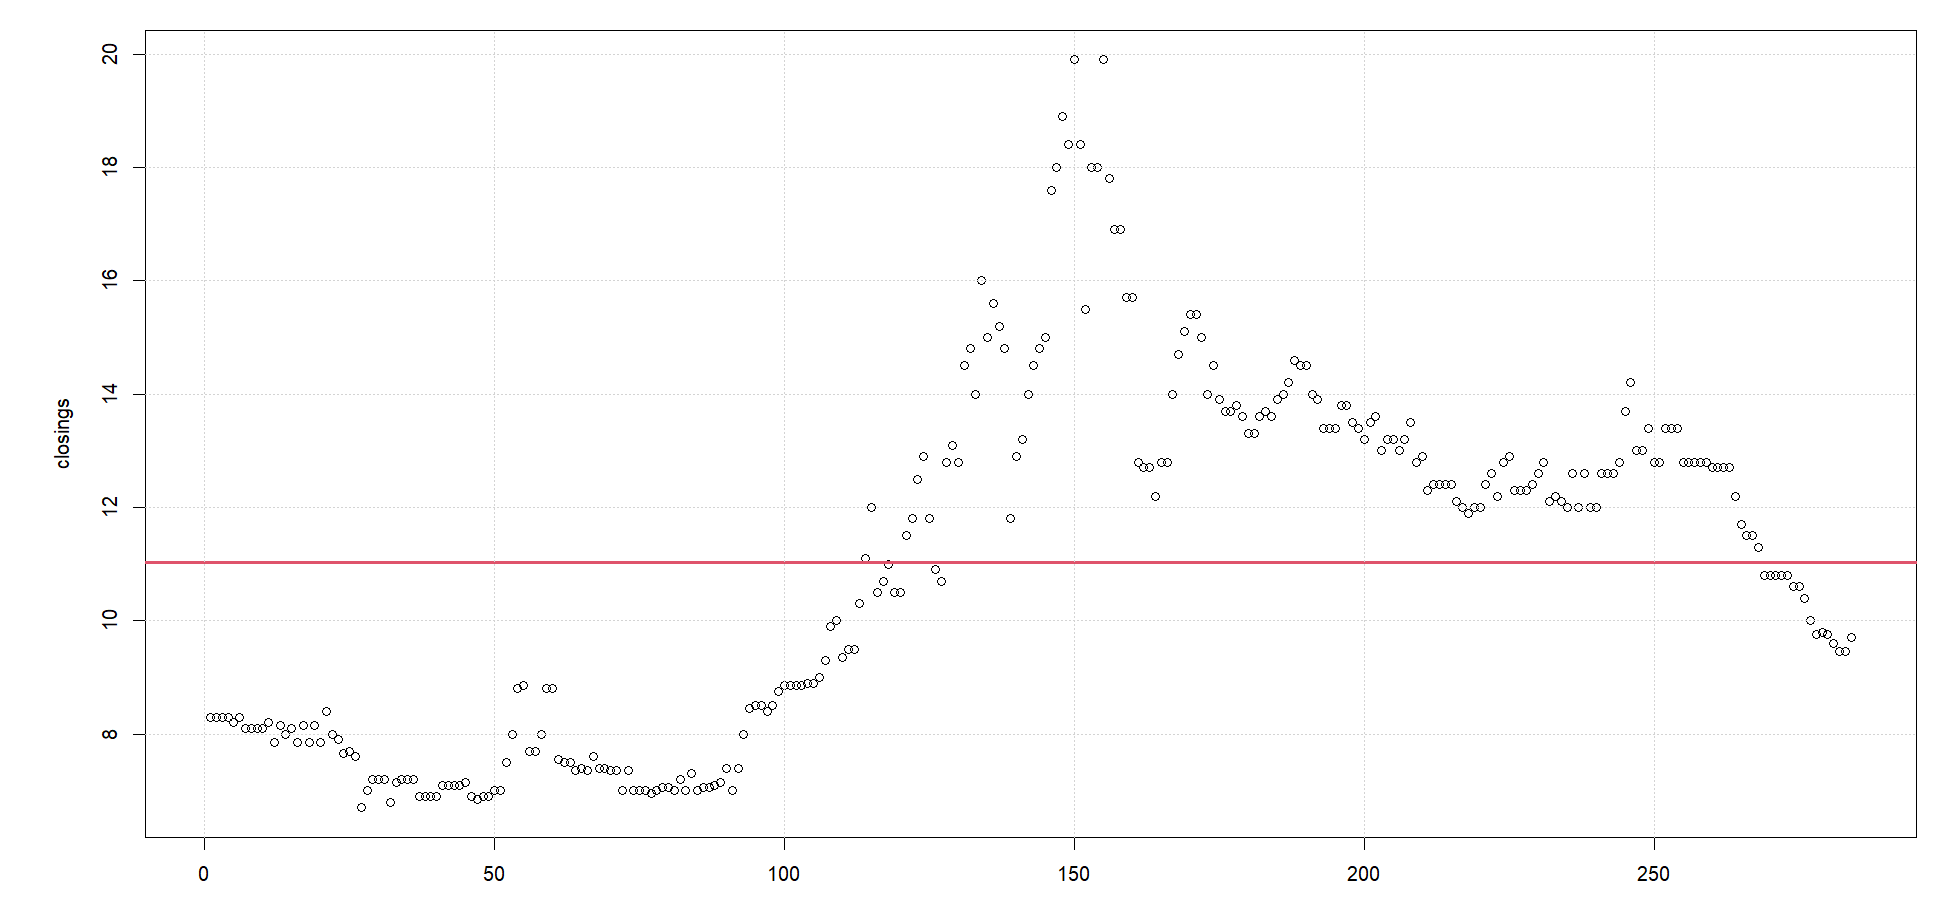
\includegraphics[width=14cm]{./Janek/zamkniecie.png}}

Poniżej przedstawiam wykres log-zwrotów wybranej spółki

\centerline{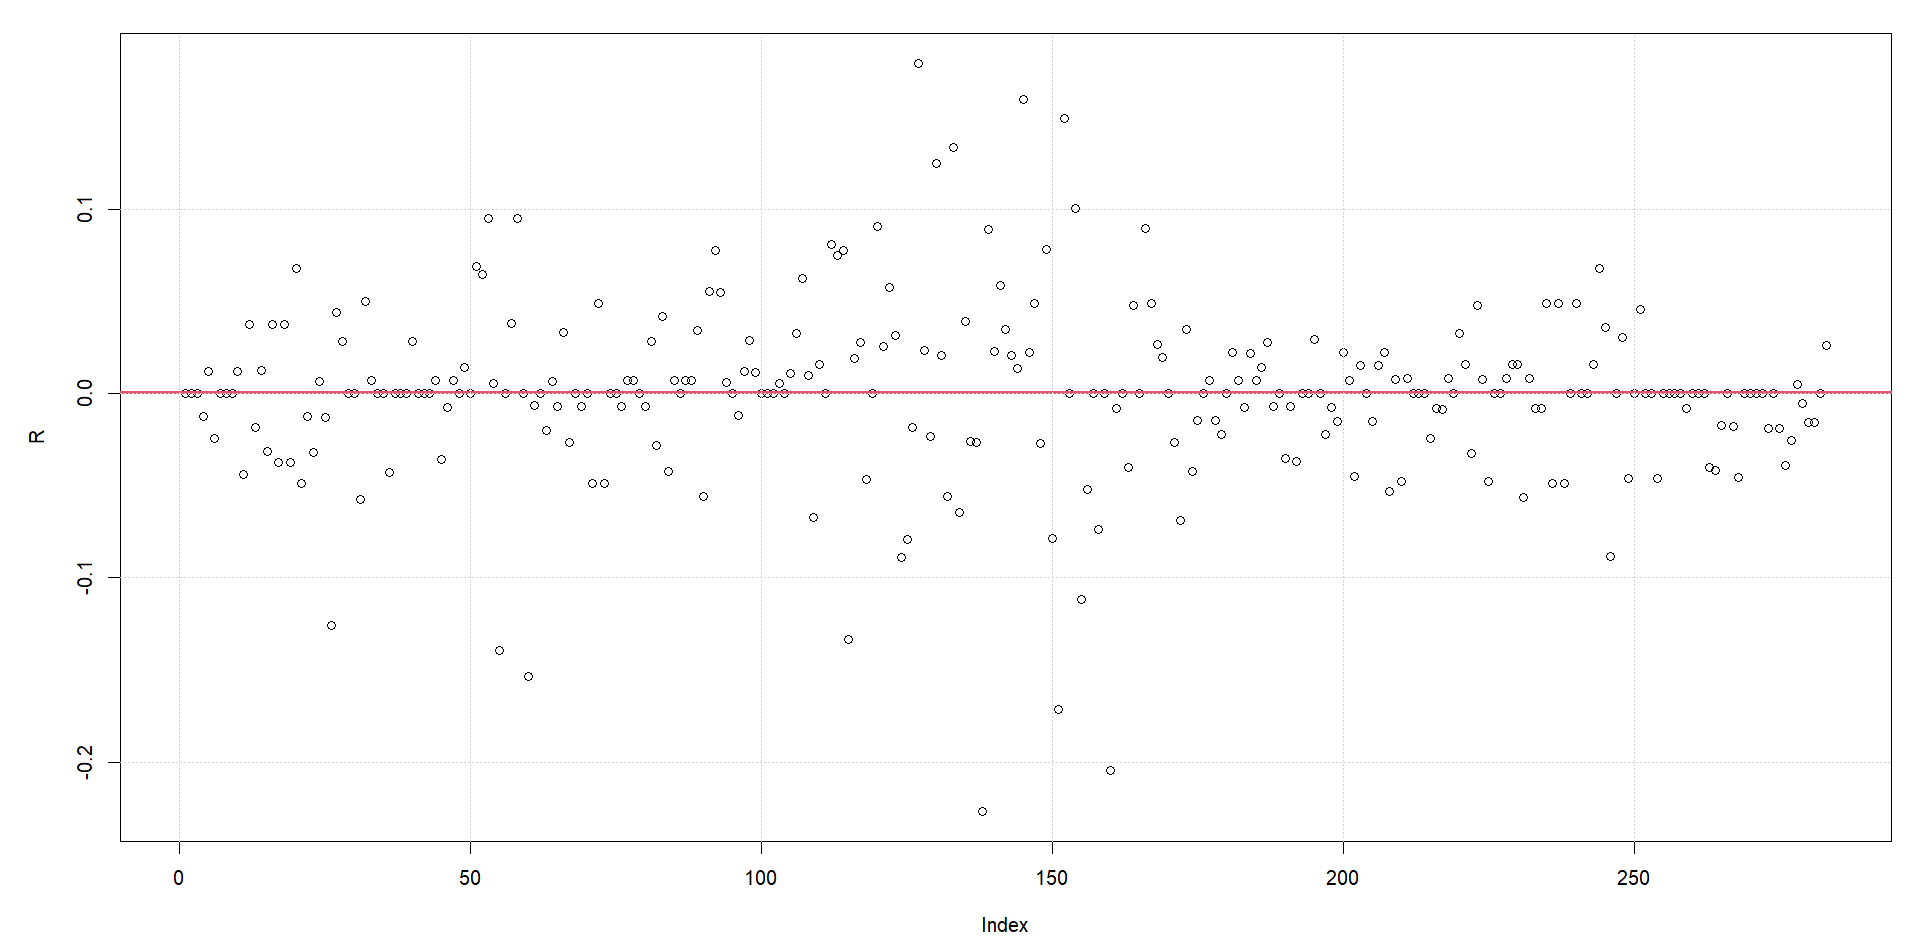
\includegraphics[width=14cm]{./Janek/logzwroty.png}}

\paragraph{Podstawowa analiza statystyczna log-zwrotów:}

Wartości log-zwrotów zostały obliczone jako różnice logarytmiczne dziennych kursów zamknięcia. Poniżej przedstawiono podstawowe statystyki log-zwrotów:
\begin{itemize}
    \item Średnia log-zwrotów: $\overline{x}_n = 0.0005507787$
    \item Wariancja log-zwrotów: $s^2_n = 0.0022445$
    \item Odchylenie standardowe log-zwrotów: $s_n = 0.04737616$
\end{itemize}

\begin{table}[h!]
\centering
\caption{Estymacja parametrów log-zwrotów}
\begin{tabular}{|c|c|c|c|c|c|}
\hline
$\overline{x}_n$ & $s^2_n$ & $s_n$ & $q(5\%)$ & $q(50\%)$ & $q(95\%)$ \\ \hline
0.0005507787 & 0.0022445 & 0.04737616 & -0.06694173 & 0.00000000 & 0.07764551 \\ \hline
\end{tabular}
\end{table}

Kwantyle 5%, 50%, i 95% przedstawiają odpowiednio wartości, poniżej których znajduje się odpowiednio 5%, 50%, i 95% log-zwrotów. Na przykład, wartość kwantyla 5% oznacza, że 5% log-zwrotów jest mniejszych od -0.0669.

\paragraph{Histogram log-zwrotów z zaznaczoną średnią i kwantylami:}

Poniżej zamieszczono histogram log-zwrotów z zaznaczonymi wartościami średniej oraz kwantyli 5%, 50% i 95%.

\centerline{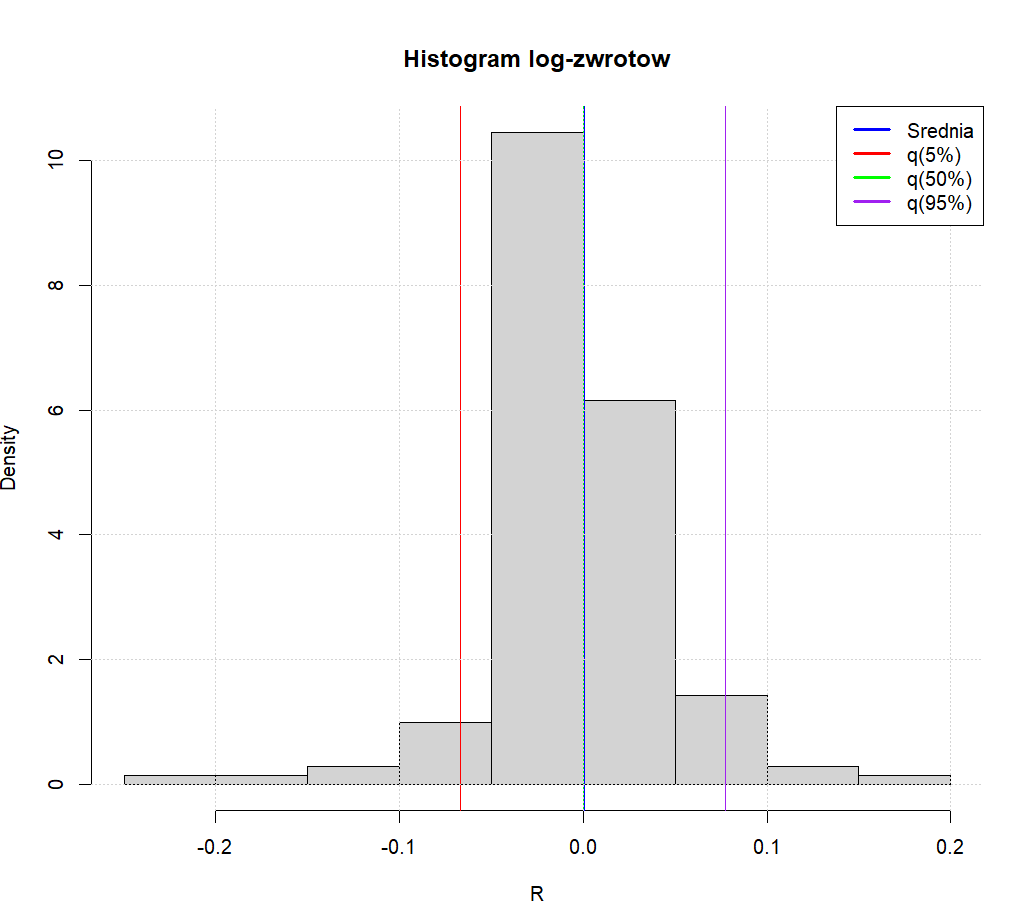
\includegraphics[width=14cm]{./Janek/histogram logzwrotow.png}}

\paragraph{Dystrybuanta empiryczna log-zwrotów:}

Estymacja dystrybuanty empirycznej dla log-zwrotów została przeprowadzona przy użyciu wzoru empirycznej dystrybuanty $F_n(x)$. Wykres dystrybuanty empirycznej log-zwrotów znajduje się poniżej.

\centerline{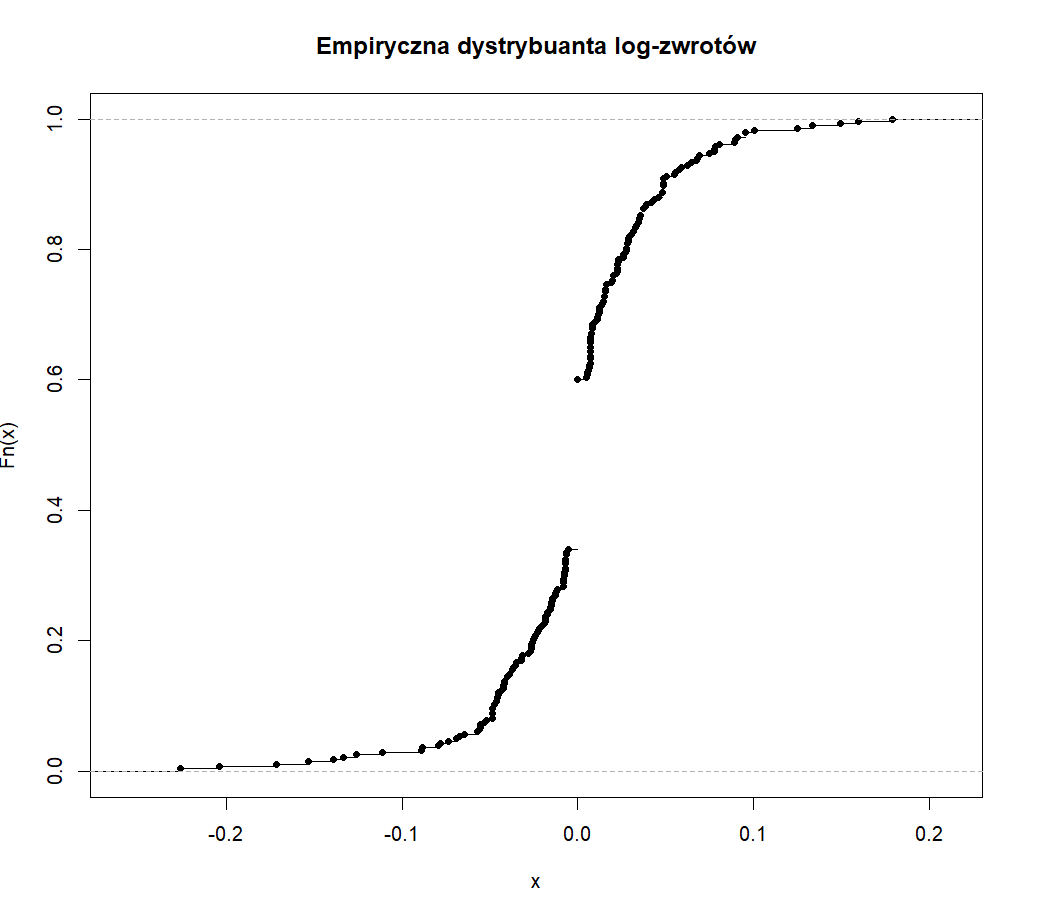
\includegraphics[width=14cm]{./Janek/empiryczna dystrybuanta.png}} 

\subsubsection{Analiza dobroci dopasowania rozkładów}

\paragraph{Estymacja parametrów rozkładu normalnego i t-Studenta:}

Parametry rozkładu normalnego i t-Studenta zostały wyestymowane przy użyciu estymatora największej wiarygodności (MLE):
\begin{itemize}
    \item Rozkład normalny: średnia = 0.0005507787, odchylenie standardowe = 0.0472923802
    \item Rozkład t-Studenta: liczba stopni swobody = 307.2041
\end{itemize}

\paragraph{Wykresy diagnostyczne:}

Poniżej przedstawiono wykresy diagnostyczne dla dopasowania rozkładów normalnego i t-Studenta do danych log-zwrotów, umożliwiające ocenę jakości dopasowania.

\centerline{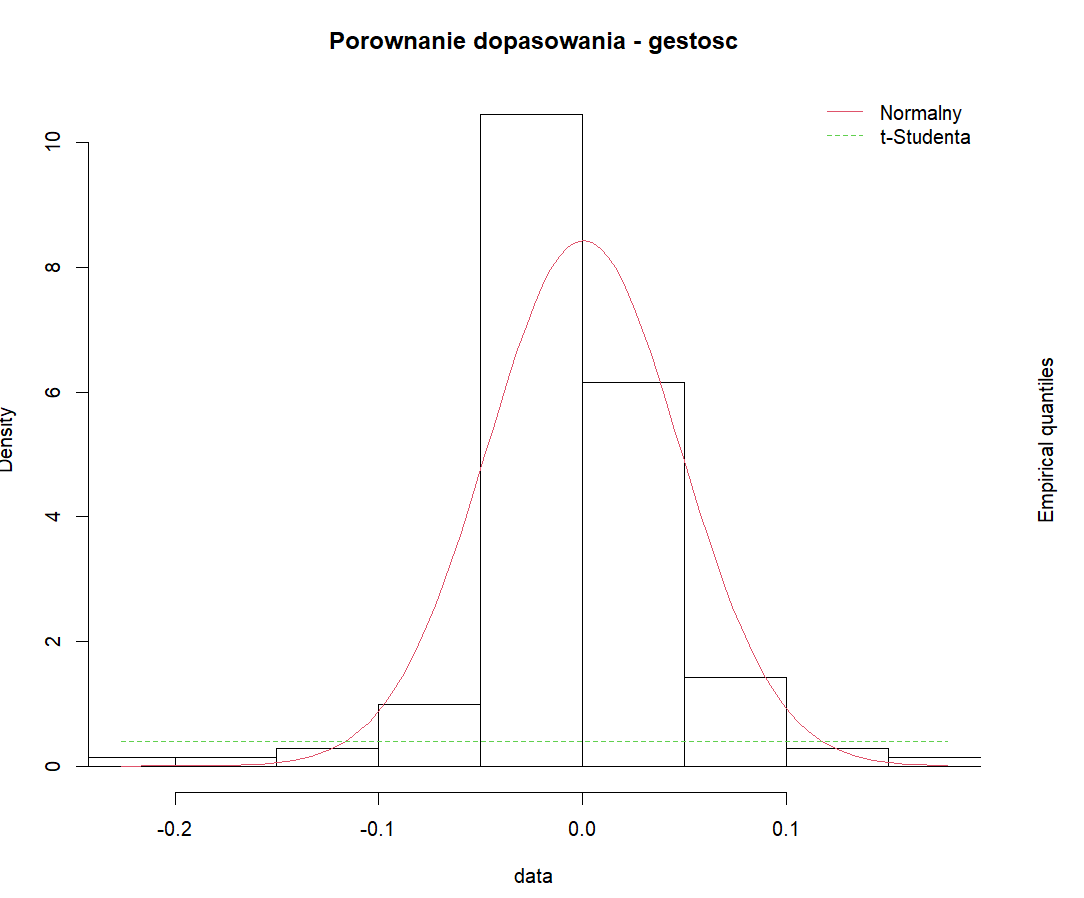
\includegraphics[width=14cm]{./Janek/dopasowanie gestosc.png}}
\centerline{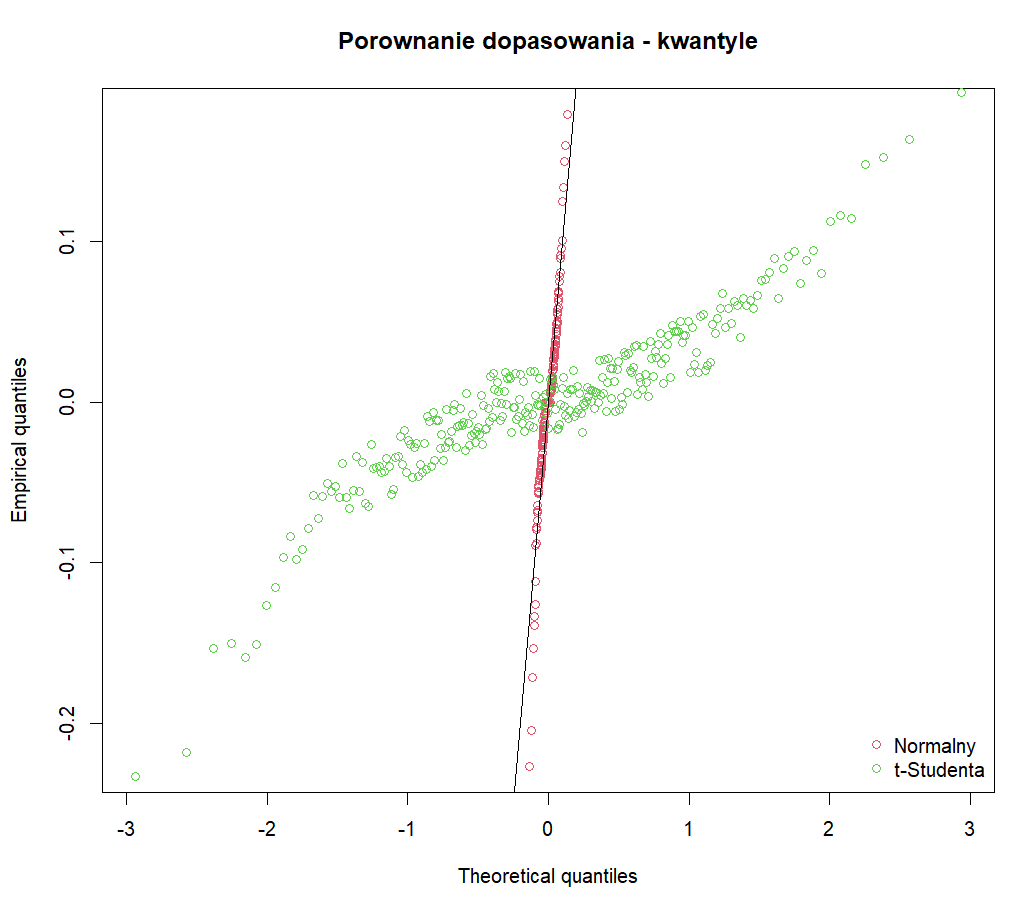
\includegraphics[width=14cm]{./Janek/dopasowanie kwantyle.png}} 
\centerline{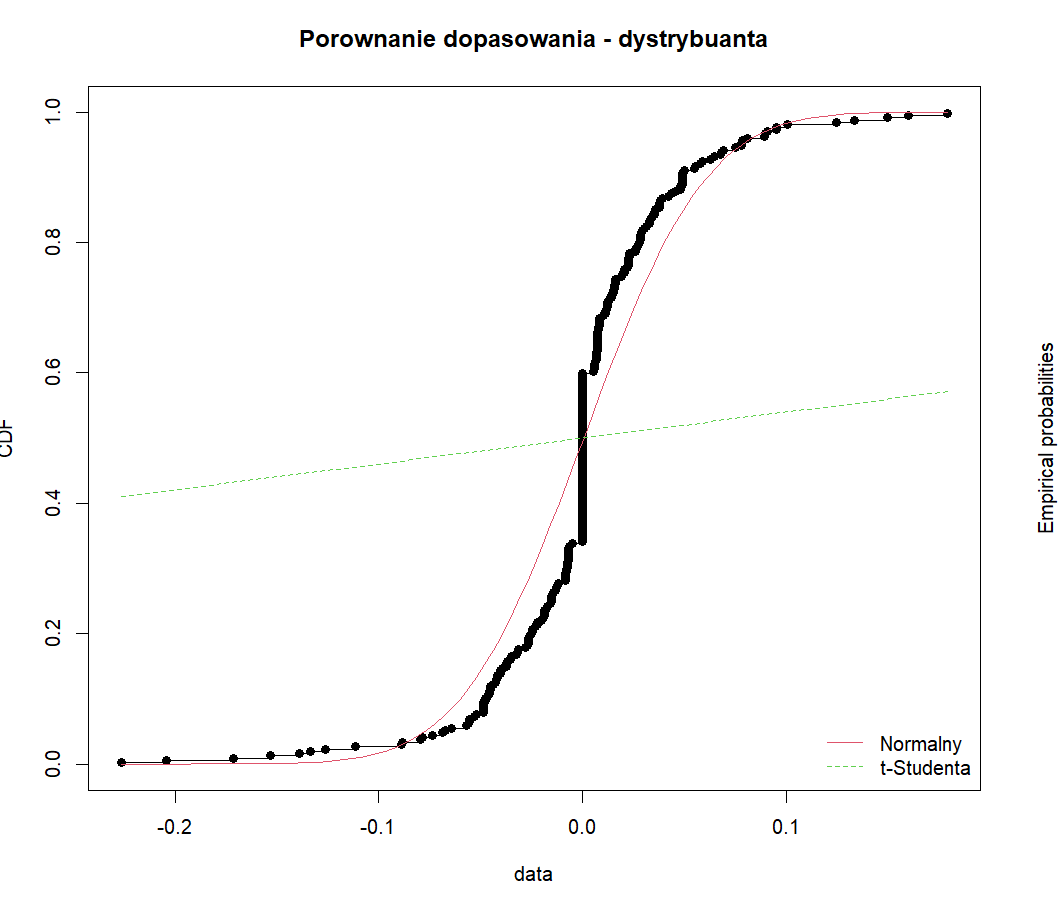
\includegraphics[width=14cm]{./Janek/dopasowanie dystrybuanta.png}}
\centerline{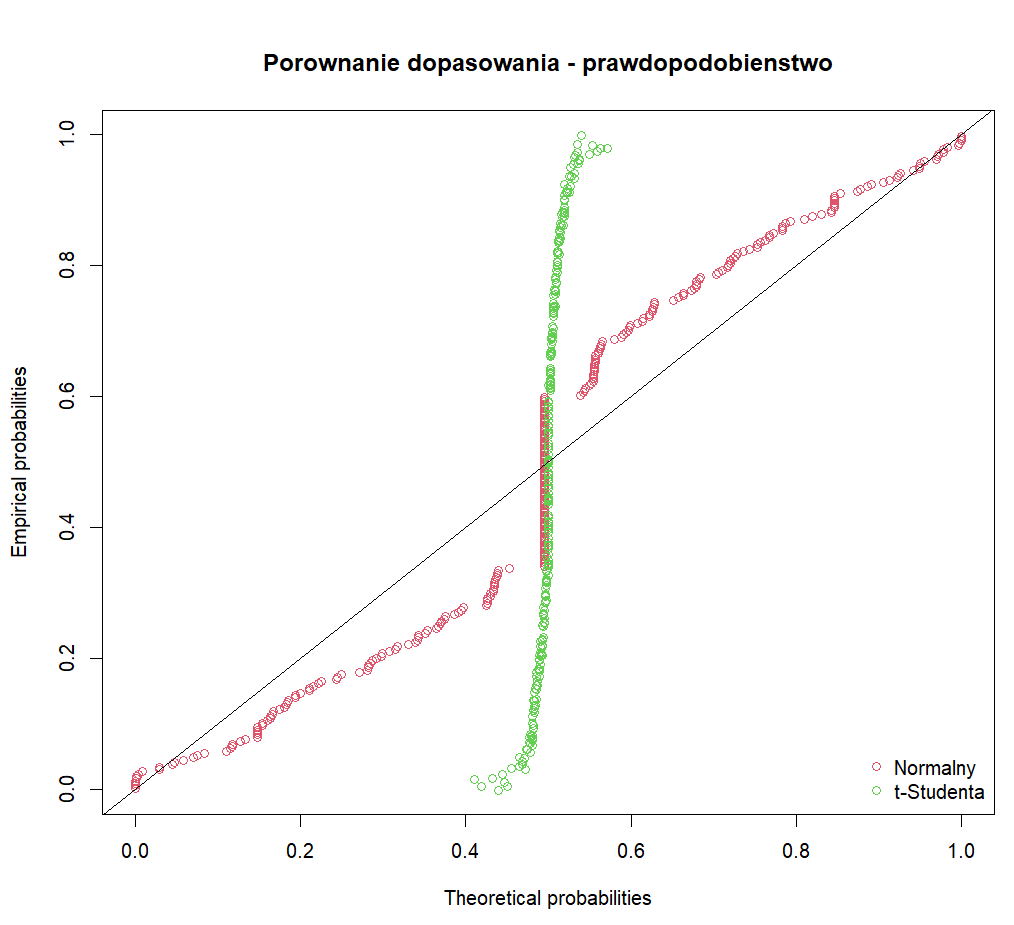
\includegraphics[width=14cm]{./Janek/dopasowanie pradopodobienstwo.png}} 

\subsection{Ocena dopasowania rozkładów}

Na podstawie wykresów diagnostycznych oraz statystyk dopasowania:
\begin{itemize}
    \item Statystyki dla rozkładu normalnego: KS = 0.1561, CM = 1.8659, AD = 9.3673, AIC = -919.9766, BIC = -912.6857
    \item Statystyki dla rozkładu t-Studenta: KS = 0.4424, CM = 21.0334, AD = 99.0999, AIC = 523.2149, BIC = 526.8603
\end{itemize}

Wyniki sugerują, że rozkład normalny lepiej dopasowuje się do danych log-zwrotów niż rozkład t-Studenta. Wybór rozkładu normalnego uzasadniają niższe wartości AIC i BIC oraz lepsze dopasowanie na wykresach diagnostycznych.

\paragraph{Test hipotezy o równości rozkładów:}

Przeprowadzono test hipotezy o równości rozkładów dla wybranego rozkładu normalnego, wykorzystując statystykę Kolmogorova-Smirnova (KS). Wyniki testu przedstawiono poniżej:

\begin{itemize}
    \item \textbf{Statystyka testowa \( D \):} Obliczona wartość wynosi \( D = 0.1561313 \). Statystyka \( D \) mierzy maksymalną różnicę pomiędzy dystrybuantą empiryczną danych a teoretyczną dystrybuantą rozkładu normalnego. Wysoka wartość \( D \) wskazuje na większą różnicę, co może sugerować, że dane nie pochodzą z badanego rozkładu.
    \item \textbf{P-wartość (\( p \)):} Obliczona p-wartość wynosi \( p = 0 \). Oznacza to, że przy założeniu prawdziwości hipotezy zerowej, prawdopodobieństwo uzyskania tak dużej lub większej różnicy \( D \) wynosi praktycznie zero. W rezultacie, hipoteza zerowa o zgodności rozkładu danych z rozkładem normalnym zostaje odrzucona na dowolnym poziomie istotności.
\end{itemize}

\textbf{Interpretacja:}
\begin{itemize}
    \item Obliczona wartość statystyki \( D \) sugeruje, że istnieją istotne różnice pomiędzy rozkładem danych a teoretycznym rozkładem normalnym. 
    \item Niska p-wartość (\( p = 0 \)) wskazuje, że te różnice są statystycznie istotne. Oznacza to, że dane najprawdopodobniej nie pochodzą z badanego rozkładu normalnego.
\end{itemize}

\subsection{Wawel}

\section{Analiza łącznego rozkładu log-zwrotów}

\end{document}